\documentclass{beamer}[10]
\usepackage{pgf}
\usepackage[english]{babel}
\usepackage[utf8]{inputenc}
\usepackage{beamerthemesplit}
\usepackage{graphics,epsfig}
\usepackage{caption}
\usepackage{subcaption}
\usepackage{url}
\usepackage{srcltx}
\usepackage{hyperref}
\usepackage{media9,graphicx}
\usepackage{multicol}
\usepackage{natbib}
\setlength{\bibsep}{4pt}
%\renewcommand*{\bibfont}{\footnotesize}

%\setbeamerfont{bibliography item}{size=\footnotesize}
%\setbeamerfont{bibliography entry author}{size=\footnotesize}
%\setbeamerfont{bibliography entry title}{size=\footnotesize}
%\setbeamerfont{bibliography entry location}{size=\footnotesize}
%\setbeamerfont{bibliography entry note}{size=\footnotesize}

\definecolor{kugreen}{RGB}{50,93,61}
\definecolor{kugreenlys}{RGB}{132,158,139}
\definecolor{kugreenlyslys}{RGB}{173,190,177}
\definecolor{kugreenlyslyslys}{RGB}{214,223,216}

\setbeamerfont{caption}{size=\tiny}
\setbeamercovered{transparent}
\mode<presentation>{}
\usetheme[numbers,totalnumber, compress,sidebarshades]{PaloAlto}


  \usecolortheme[named=kugreen]{structure}
  \useinnertheme{circles}
  \usefonttheme[onlymath]{serif}
  \setbeamercovered{transparent}
  \setbeamertemplate{blocks}[rounded][shadow=true]


\useoutertheme{smoothbars} 

%\AtBeginSection[]
%{
%	\begin{frame}
%		\frametitle{Table of Contents}
%		\tableofcontents[currentsection]
%	\end{frame}
%}

\AtBeginSubsection[]{
	\begin{frame}
		\frametitle{Table of Contents}
		\tableofcontents[currentsubsection]
	\end{frame}
}



\title{Laki to Tambora}
%\author{Thea Quistgaard}
\subtitle{\small \textit{Pattern Recognition in High Resolution Volcanic and Isotopic Signals}}
\author[T. Quistgaard]{Thea Quistgaard\inst{1}}
%\author{Supervisor: Klaus Mosegaard}
\institute[UCPH]{\inst{1}University of Copenhagen}
\logo{\includegraphics[width=0.8cm]{KULogo.eps}}

\begin{document}
{\setbeamertemplate{footline}[frame number]
\frame{\titlepage \vspace{-0.5cm}	
}}

\begin{frame}{Outline of talk}
	\tableofcontents
\end{frame}


%\setbeamertemplate{footline}[frame number]
\addtocounter{page}{-1}

\section{So Far...}

\subsection{Water Isotopes}

\frame{
\frametitle{Water Isotopes in Ice Cores}
\begin{figure}[h]
	\centering
	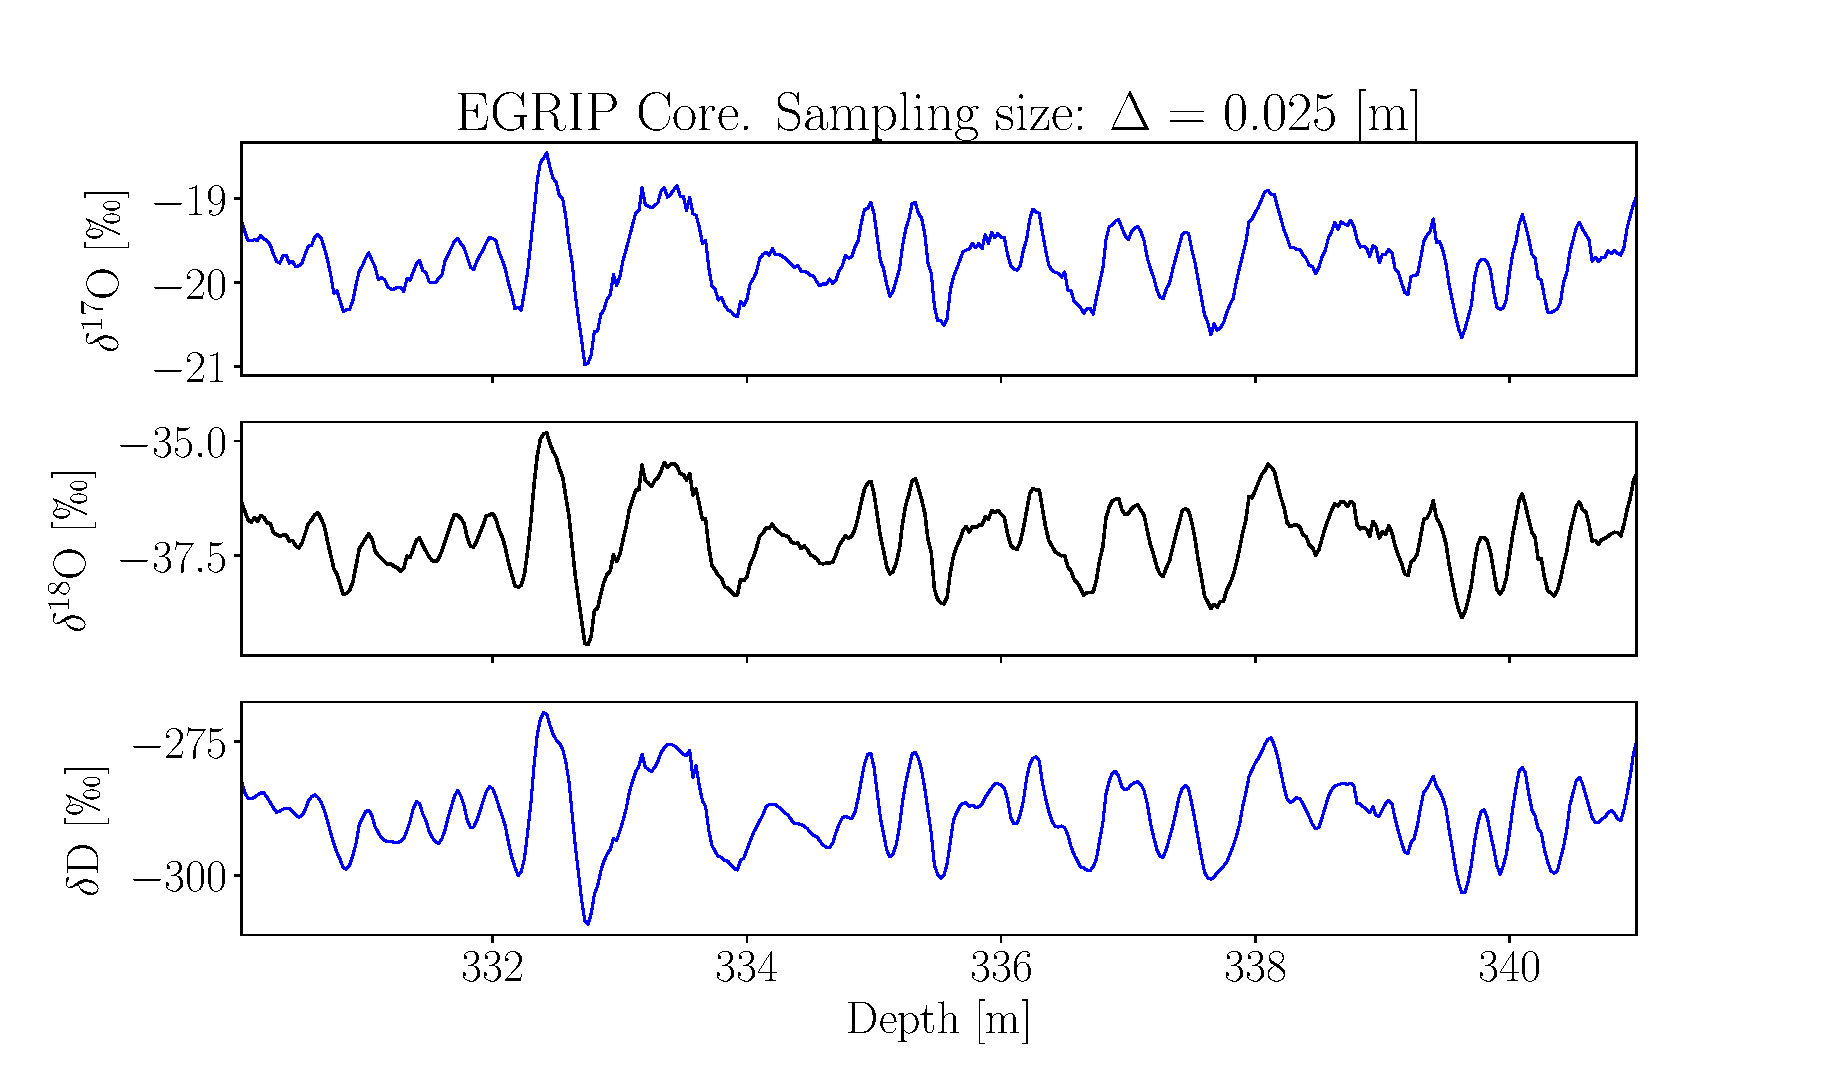
\includegraphics[width=0.9\textwidth]{d17d18dD_ExamplesEGRIP.eps}
	\label{fig:d17d18dD_ExamplesEGRIP}
	\caption{Examples of three water isotopes measured from the EGRIP core in Greenland.}
\end{figure}
}


\frame{
	\frametitle{Diffusion in Firn}
\begin{itemize}
	\item<1-6> Fick's $2^{\text{nd}}$ law:
	\begin{equation}
		\frac{\partial\delta}{\partial t} = D(t)\frac{\partial^2\delta}{\partial z^2} - \dot{\epsilon}_z (t) z \frac{\partial\delta}{\partial z}
		\label{Eq:Ficks2ndLaw}
	\end{equation}
	\onslide<2>{with solution}
	\onslide<2-6>{
	\begin{equation}
		\delta(z) = S(z)[\delta'(z)*\mathcal{G}(z)]
	\end{equation}}
	\onslide<3>{where $\delta(z)$ is the measured signal, $\delta'(z)$ is the initial isotopic signal}
	\onslide<4-6>{
	\begin{equation}
		\mathcal{G}(z) = \frac{1}{\sigma\sqrt{2\pi}}e^{-\frac{z^2}{2\sigma^2}}, \quad \text{a Gaussian filter,}
	\end{equation}
	}
	\onslide<5>{and}
	\onslide<5-6>{
	\begin{equation}
		\mathcal{S}(z) = e^{\int_{0}^{z}\dot{\epsilon_z}(z')dz'}, \quad \text{the thinning function}
	\end{equation}
	}
\end{itemize}
}

\frame{
	\frametitle{Actual Total Diffusion}
\onslide<1->{
Total diffusion in ice and firn
\begin{equation}
	\sigma^2_{\text{tot}} = [S(z)\sigma_{\text{firn}}]^2 + \sigma^2_{\text{ice}}(z)
\end{equation}}

\onslide<2->{Giving an actual measured diffusion length of
	\begin{equation}
		\hat{\sigma}_i^2 = \sigma_{\text{firn}}^2\,S(z) + \sigma_{\text{ice}}^2 + \sigma_{\text{dis}}^2
	\end{equation}
	with
	\begin{equation}
		\sigma_{\text{dis}}^2 = \frac{2\Delta^2}{\pi^2}\ln\left(\frac{\pi}{2}\right)
\end{equation}}
	
}

\subsection{Data}

\frame{
	\frametitle{Example Data: Site A}
	
	\begin{figure}
		\centering
		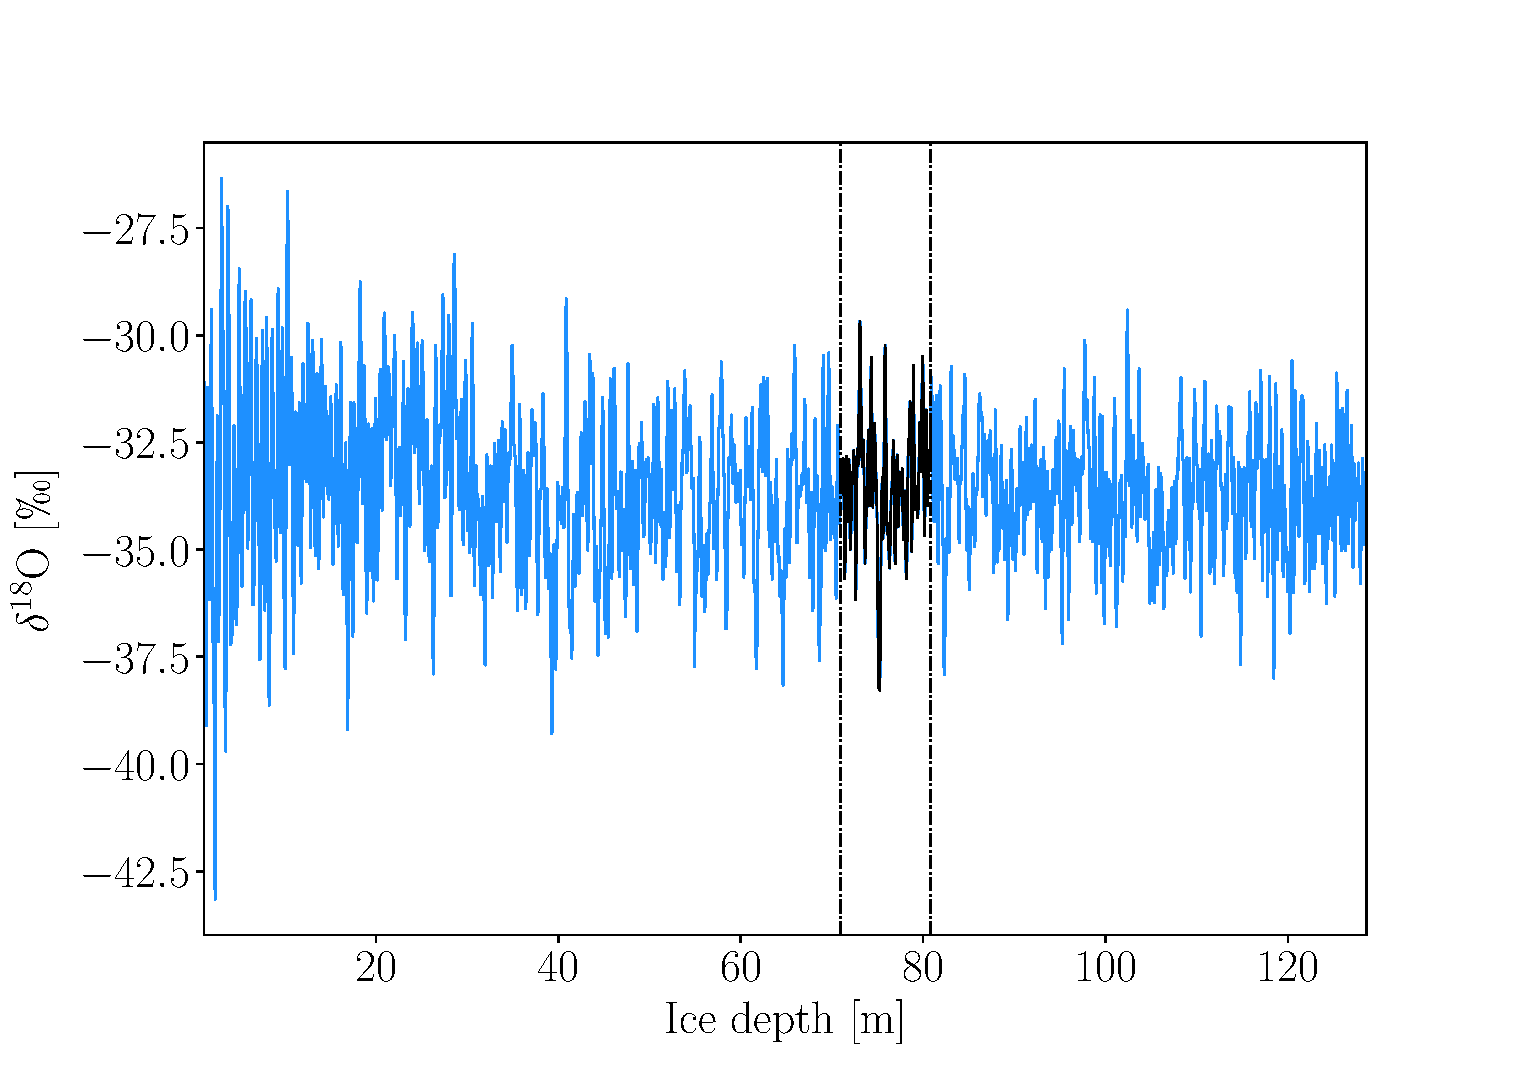
\includegraphics[width=0.9\textwidth]{SiteA_FullIso.eps}
		\caption[Site A isotopes]{Example data from Alphabet Core drilled at site A near Crête.}
		\label{fig:SiteA_FullIso}
	\end{figure}
	
	
}

\frame{
	\frametitle{Unevenly Sampled Data: Spline Interpolation}
	\begin{figure}
		\centering
		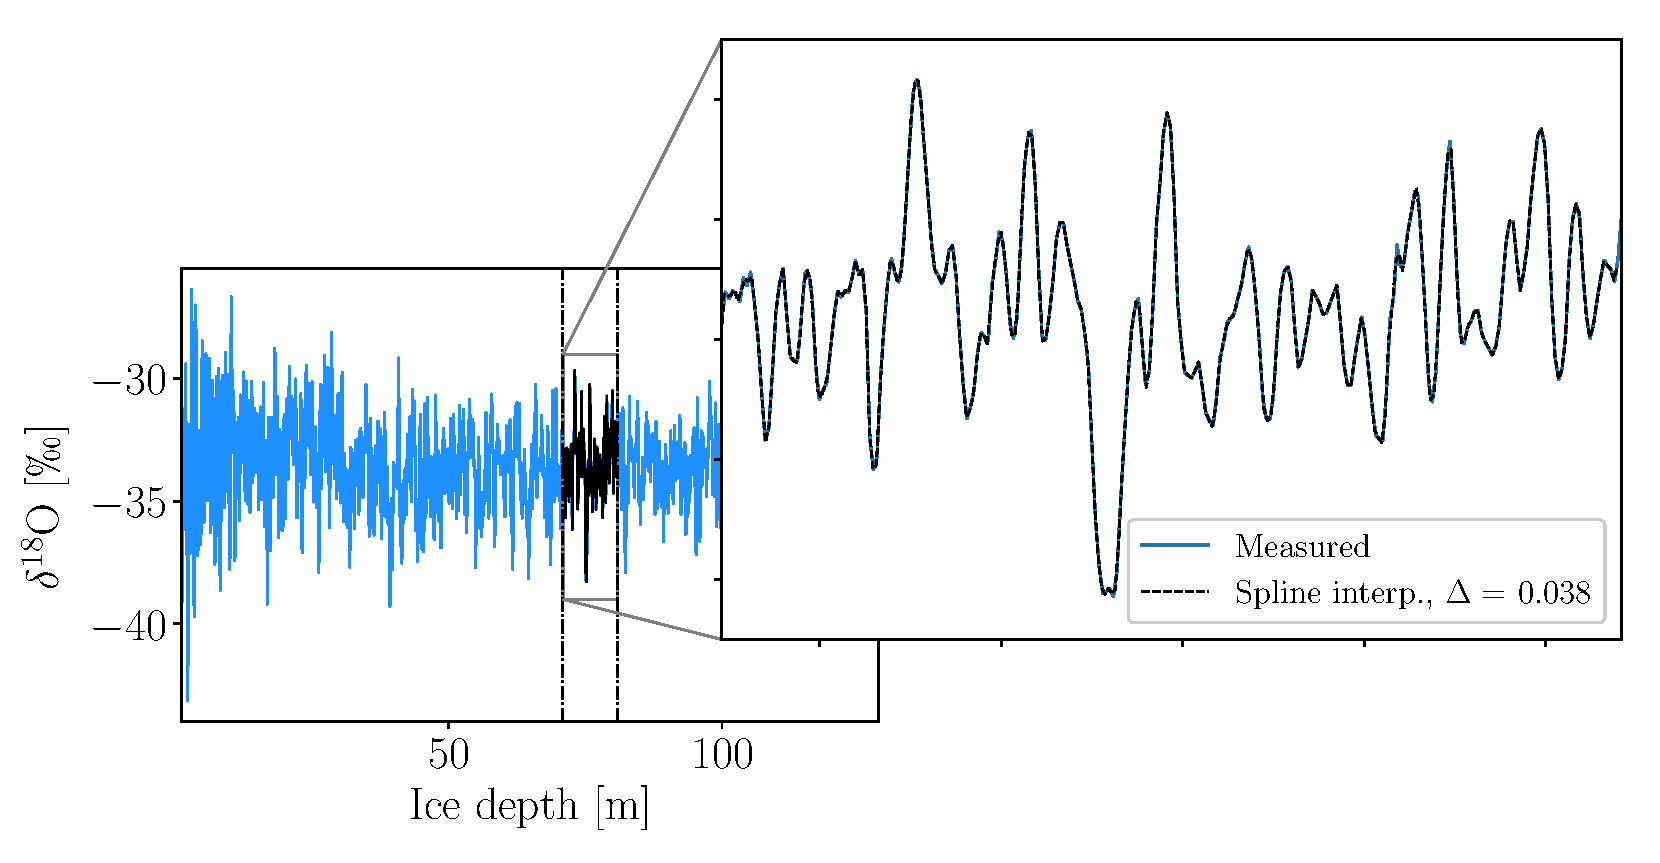
\includegraphics[width=\textwidth]{SiteA_Iso_int_Inset.eps}
		\caption[Site A Laki to Tambora isotopes, w. inset]{Example data from Alphabet Core drilled at site A near Crête. Shows zoom in of data from Laki to Tambora along with spline interpolated data.}
		\label{fig:SiteA_Iso_int_Inset}
	\end{figure}	
	
}



\frame{
	\frametitle{Community Firn Model}

	\begin{figure}
		\centering
		\begin{subfigure}{.45\textwidth}
			\centering
			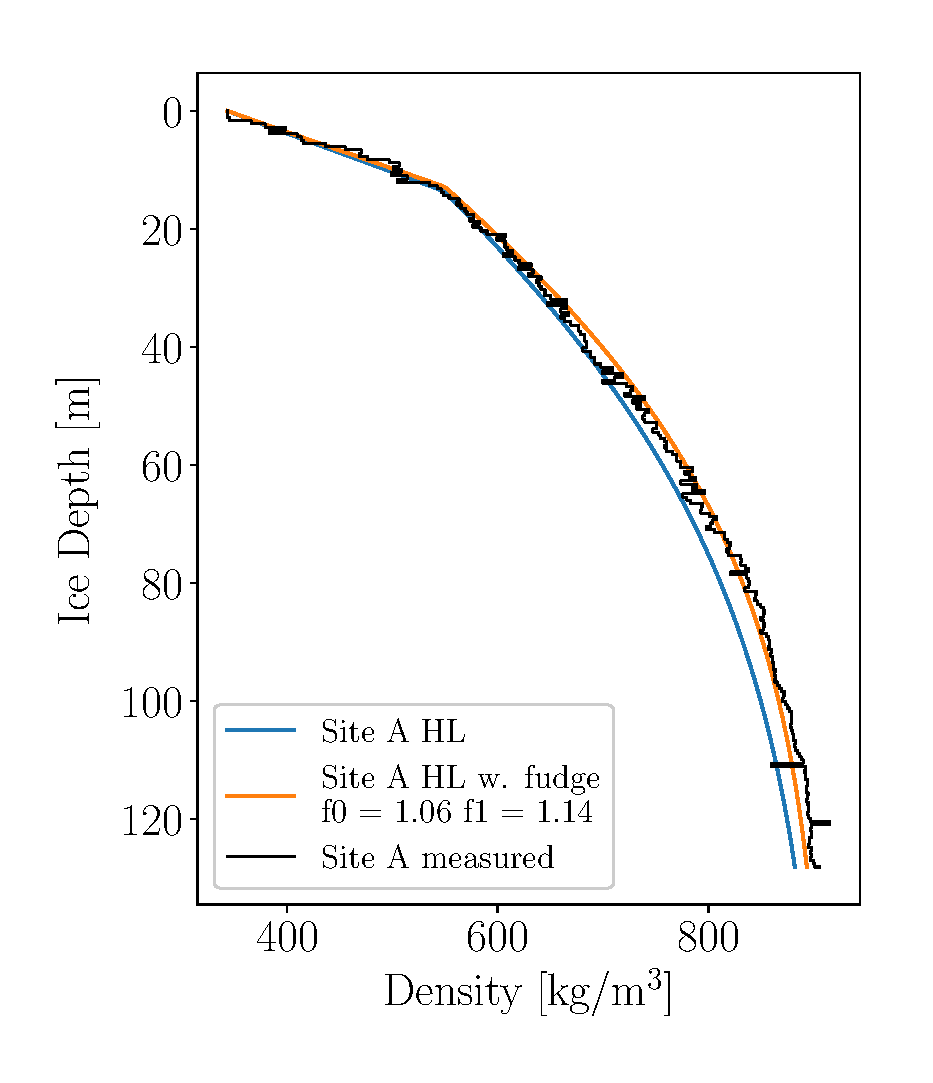
\includegraphics[width=\linewidth]{SiteA_HLdensity.eps}
			\caption[Density-depth profile, Site A]{\tiny Density-depth profiles based on analytical Herron-Langway model. Black is empirical data, blue is purely analytical fit and orange is fudged analytical fit}
			\label{fig:SiteA_HLdensity}
		\end{subfigure}%
		~
		\begin{subfigure}{.45\textwidth}
			\centering
			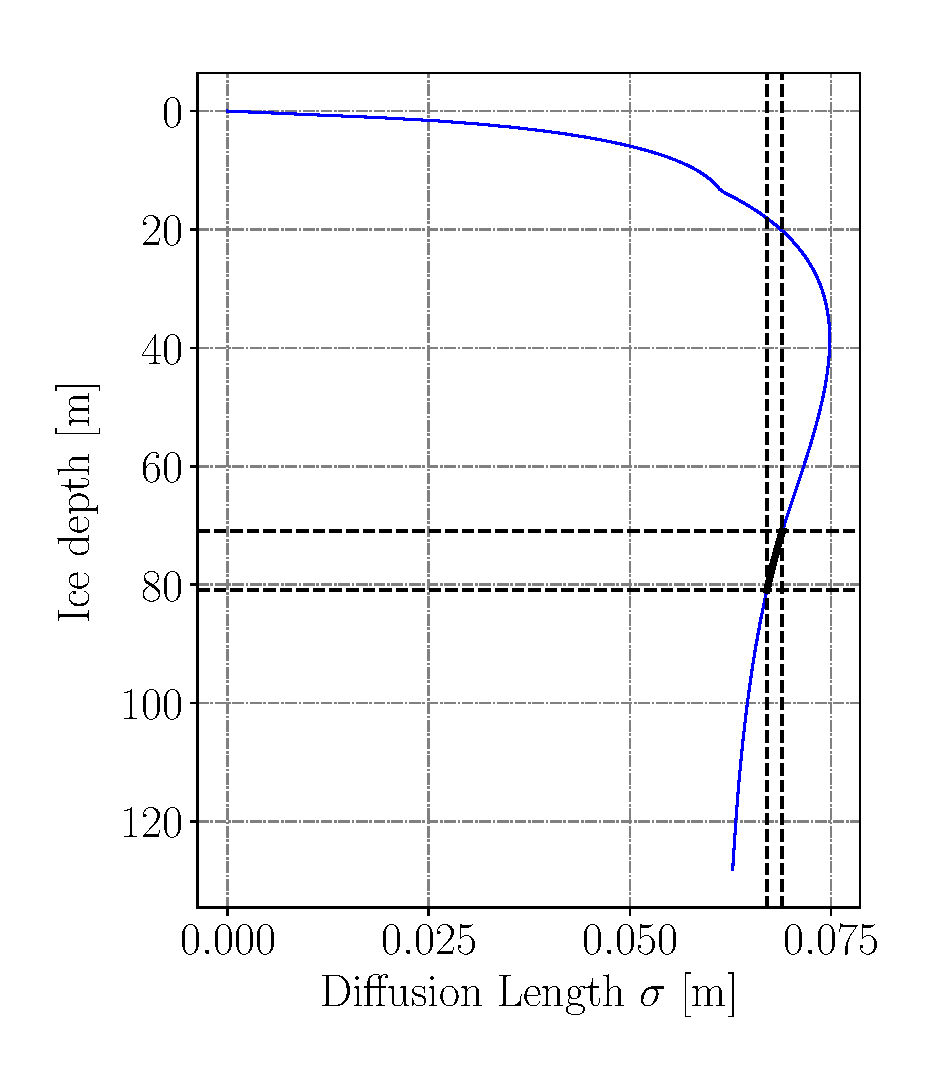
\includegraphics[width=\linewidth]{SiteA_DiffLen.eps}
			\caption[Diffusion length profile, Site A]{\tiny Modeled diffusion length profile based on empirically computed density profile. Black dashed lines indicate ice depth corresponding to date Laki and Tambora eruptions.}
			\label{fig:SiteA_DiffLen}
		\end{subfigure}
%		\caption{A figure with two subfigures}
		\label{fig:CFM}
	\end{figure}
}





\subsection{Volcanic Horizons}

\frame{
	\frametitle{Laki and Tambora}
	\begin{itemize}
		\item \textbf{Electrical Conductivity Measurements (ECM)}
		\item \textbf{Dielectric Profiling (DEP)}
	\end{itemize}
	\begin{figure}
		\centering
		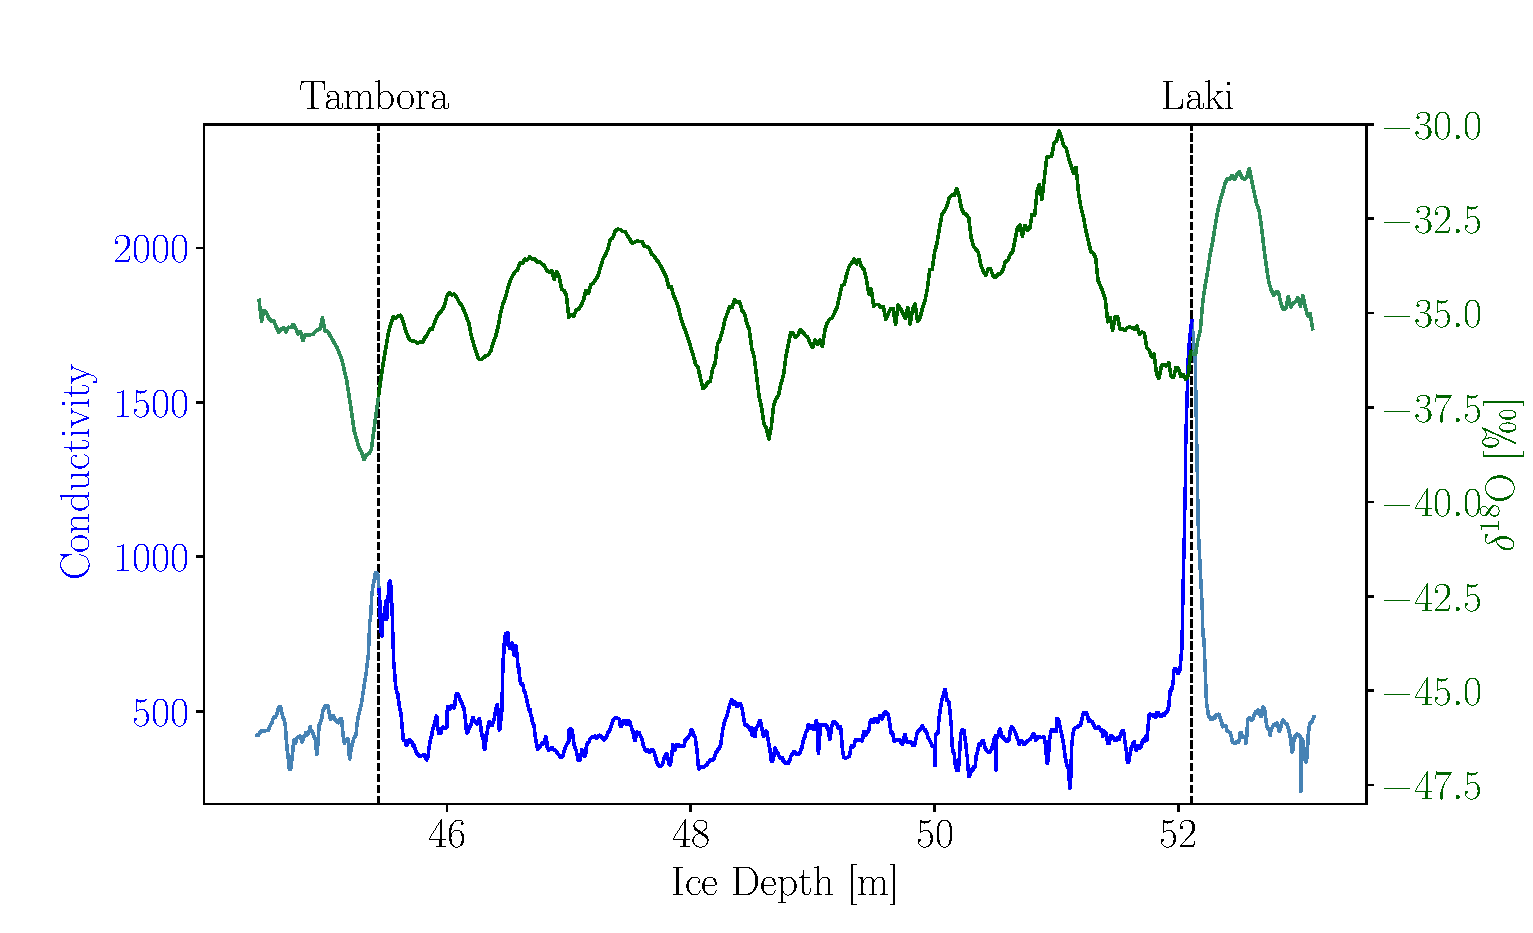
\includegraphics[width=\textwidth]{B22_DEPexample.eps}
		\caption[DEP Laki to Tambora, Core B22]{Example of volcanic horizons used for dating of cores, core B22.}
		\label{fig:B22_DEPexample}
	\end{figure}	
}

\subsection{Back Diffusion}

\begin{frame}  
	\frametitle{Spectral Analysis with DCT}
	\begin{tabular}{cl}  
		\begin{tabular}{c}
			\onslide<1->{
			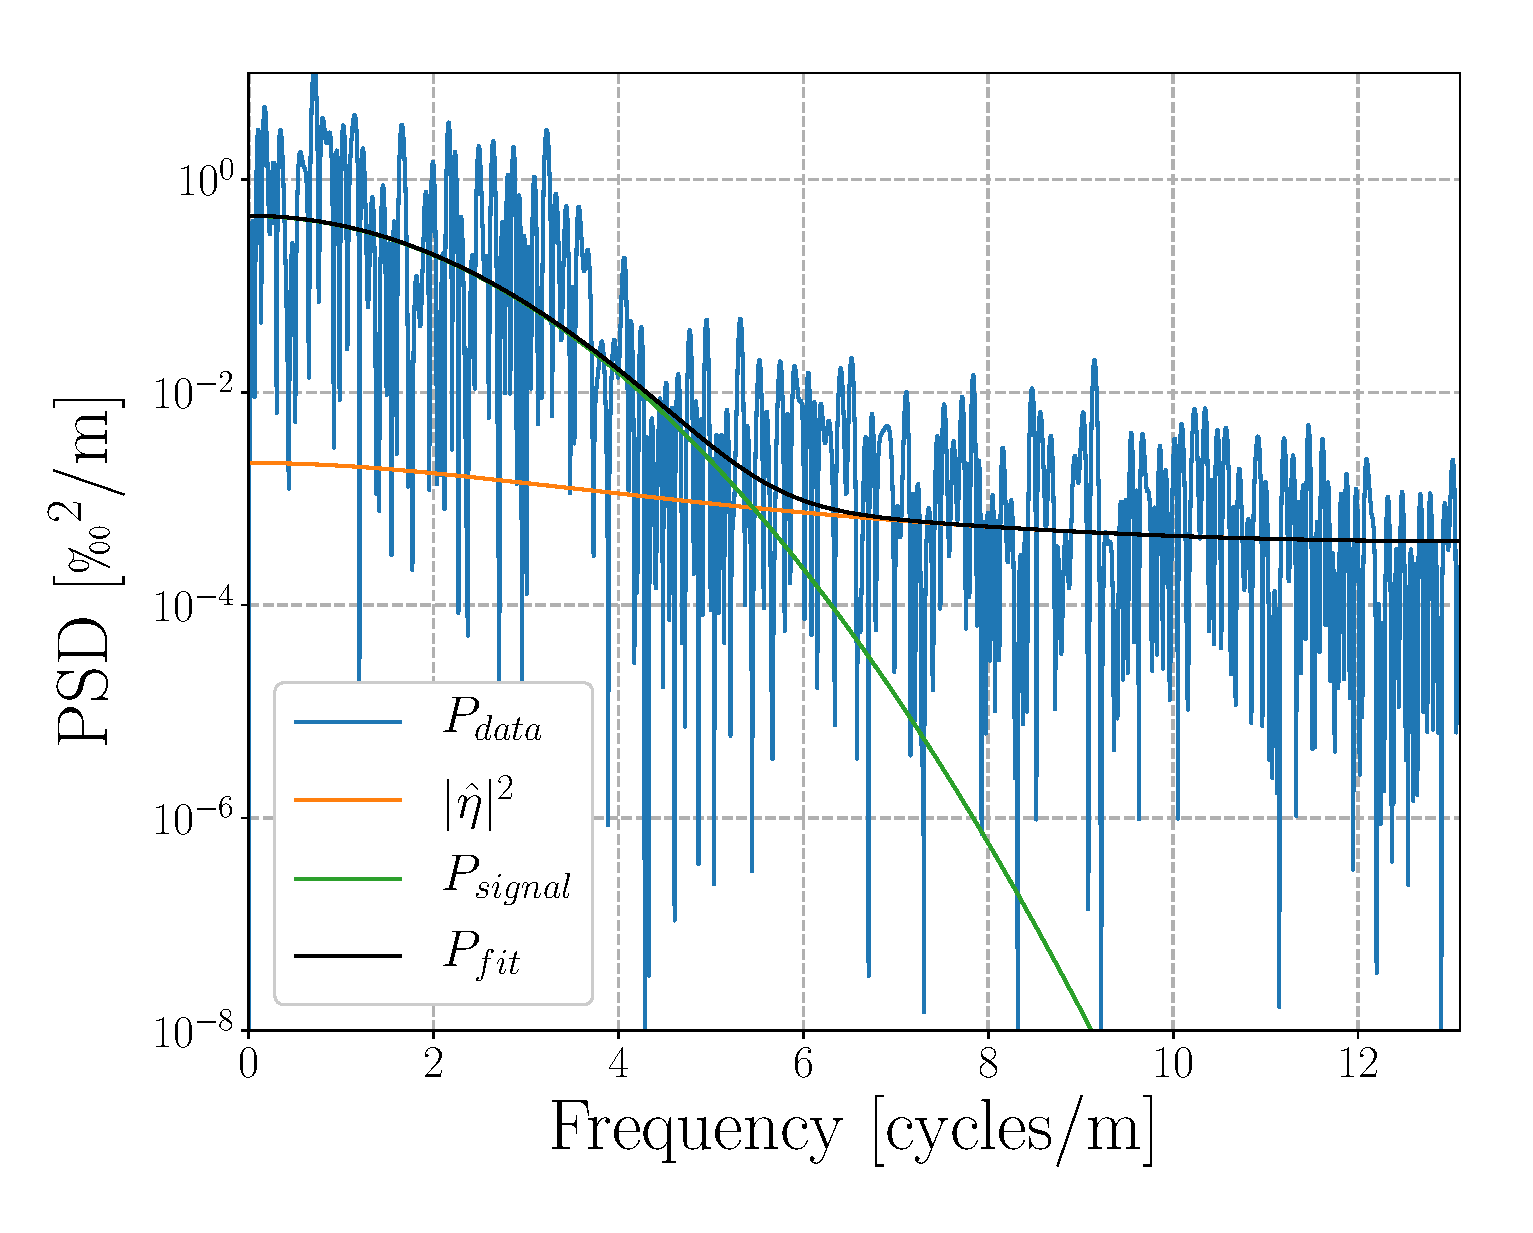
\includegraphics[height=4.5cm, width=5.6cm]{SiteA_PSD.eps}}
		\end{tabular}
		& \begin{tabular}{l}
			\parbox{0.01\linewidth}{\scriptsize %  change the parbox width as appropiate
				\onslide<2-4>{
				\begin{equation*}
					P_{\text{tot}} = P_{\text{signal}} + |\hat{\eta}|^2
				\end{equation*}}
				\onslide<3-4>{
				\begin{equation*}
					|\hat{\eta}|^2 = \frac{\sigma_{\eta}^2\Delta}{|1-a_1 e^{-ik\Delta}|^2}
				\end{equation*}}
%				\onslide<4>{
%				\begin{equation*}
%					P_{\text{signal}} = P_0 e^{-k^2\sigma^2}
%				\end{equation*}}			
			\onslide<4->{\small
			\begin{equation*}
					P_{\text{signal}} = P_0 e^{-k^2\alert<5>{\sigma^2}}
			\end{equation*}}
			}
			
		\end{tabular}  \\
	\end{tabular}
\end{frame}

%\frame{
%	\frametitle{Spectral Analysis: Discrete Cosine Transform}
	
%\begin{figure}
%	\centering
%	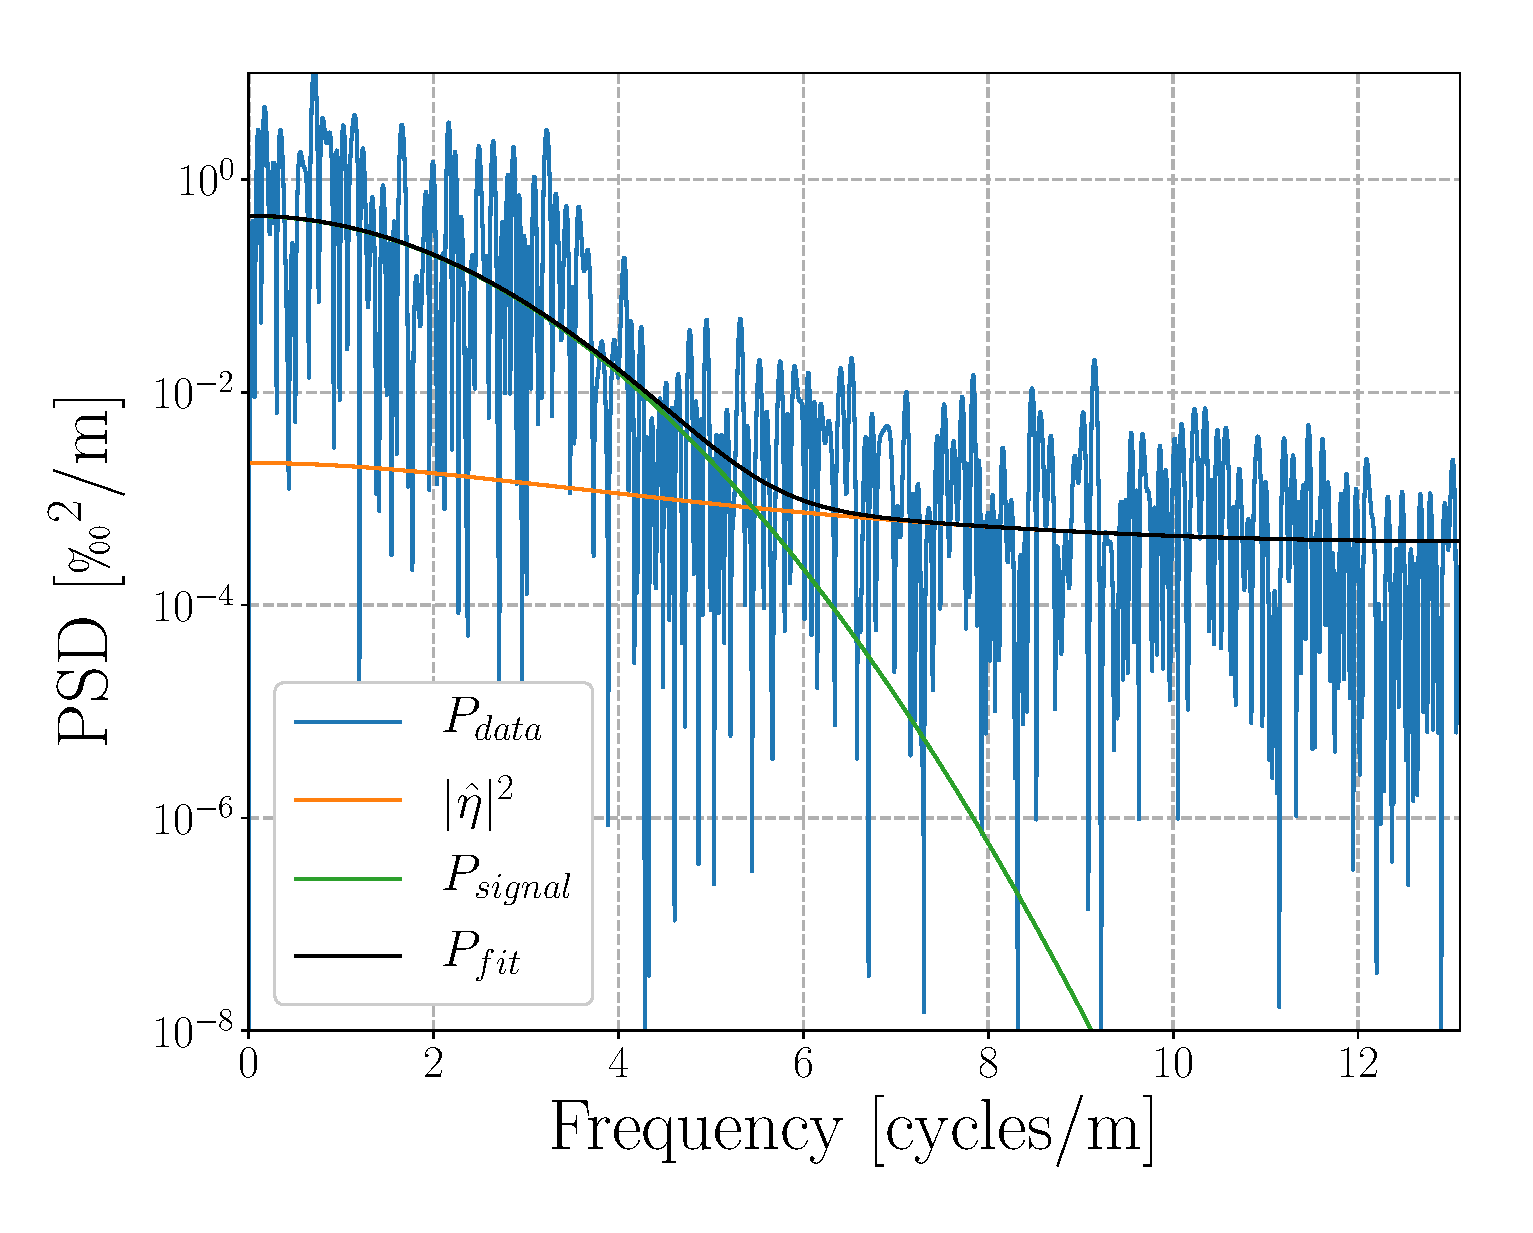
\includegraphics[width=0.7\linewidth]{SiteA_PSD.eps}
%	\caption[PSD Laki to Tambora Site A]{Power Spectral Density (PSD) of site A, L to T, data(blue) with fitted noise(orange), signal(gree) and noise plus signal(black).}
%	\label{fig:SiteA_PSD}
%\end{figure}
%}

%\frame{
%	\frametitle{Signal and Noise Fitting}
%	
%}


\frame{
	\frametitle{Diffusion Lengths and Transfer Functions}
	\onslide<1->{
	\begin{equation}
		\tilde{\delta}_{\text{meas}} = \tilde{\delta}_{\text{init}}\cdot \tilde{M} \Leftrightarrow \tilde{\delta}_{\text{init}} = \tilde{\delta}_{\text{meas}}\cdot \tilde{M}^{-1}
	\end{equation}}
	\onslide<2>{Add an optimal Wiener filter to enhance signal and minimize noise:}
	\onslide<2->{
	\begin{equation}
		\tilde{F} = \frac{P_{\text{signal}}}{P_{\text{signal}} + |\hat{\eta}|^2}
	\end{equation}}
	\onslide<3>{yielding a restoration filter as}
	\onslide<3-4>{
	\begin{equation}
		\tilde{\delta}_{\text{init}} = \tilde{\delta}_{\text{meas}}\cdot \tilde{F}\cdot \tilde{M}^{-1} = \tilde{\delta}_{\text{meas}}\cdot \tilde{R}
	\end{equation}}
}

\frame{
	\frametitle{Filtering}
	
\begin{figure}
	\centering
	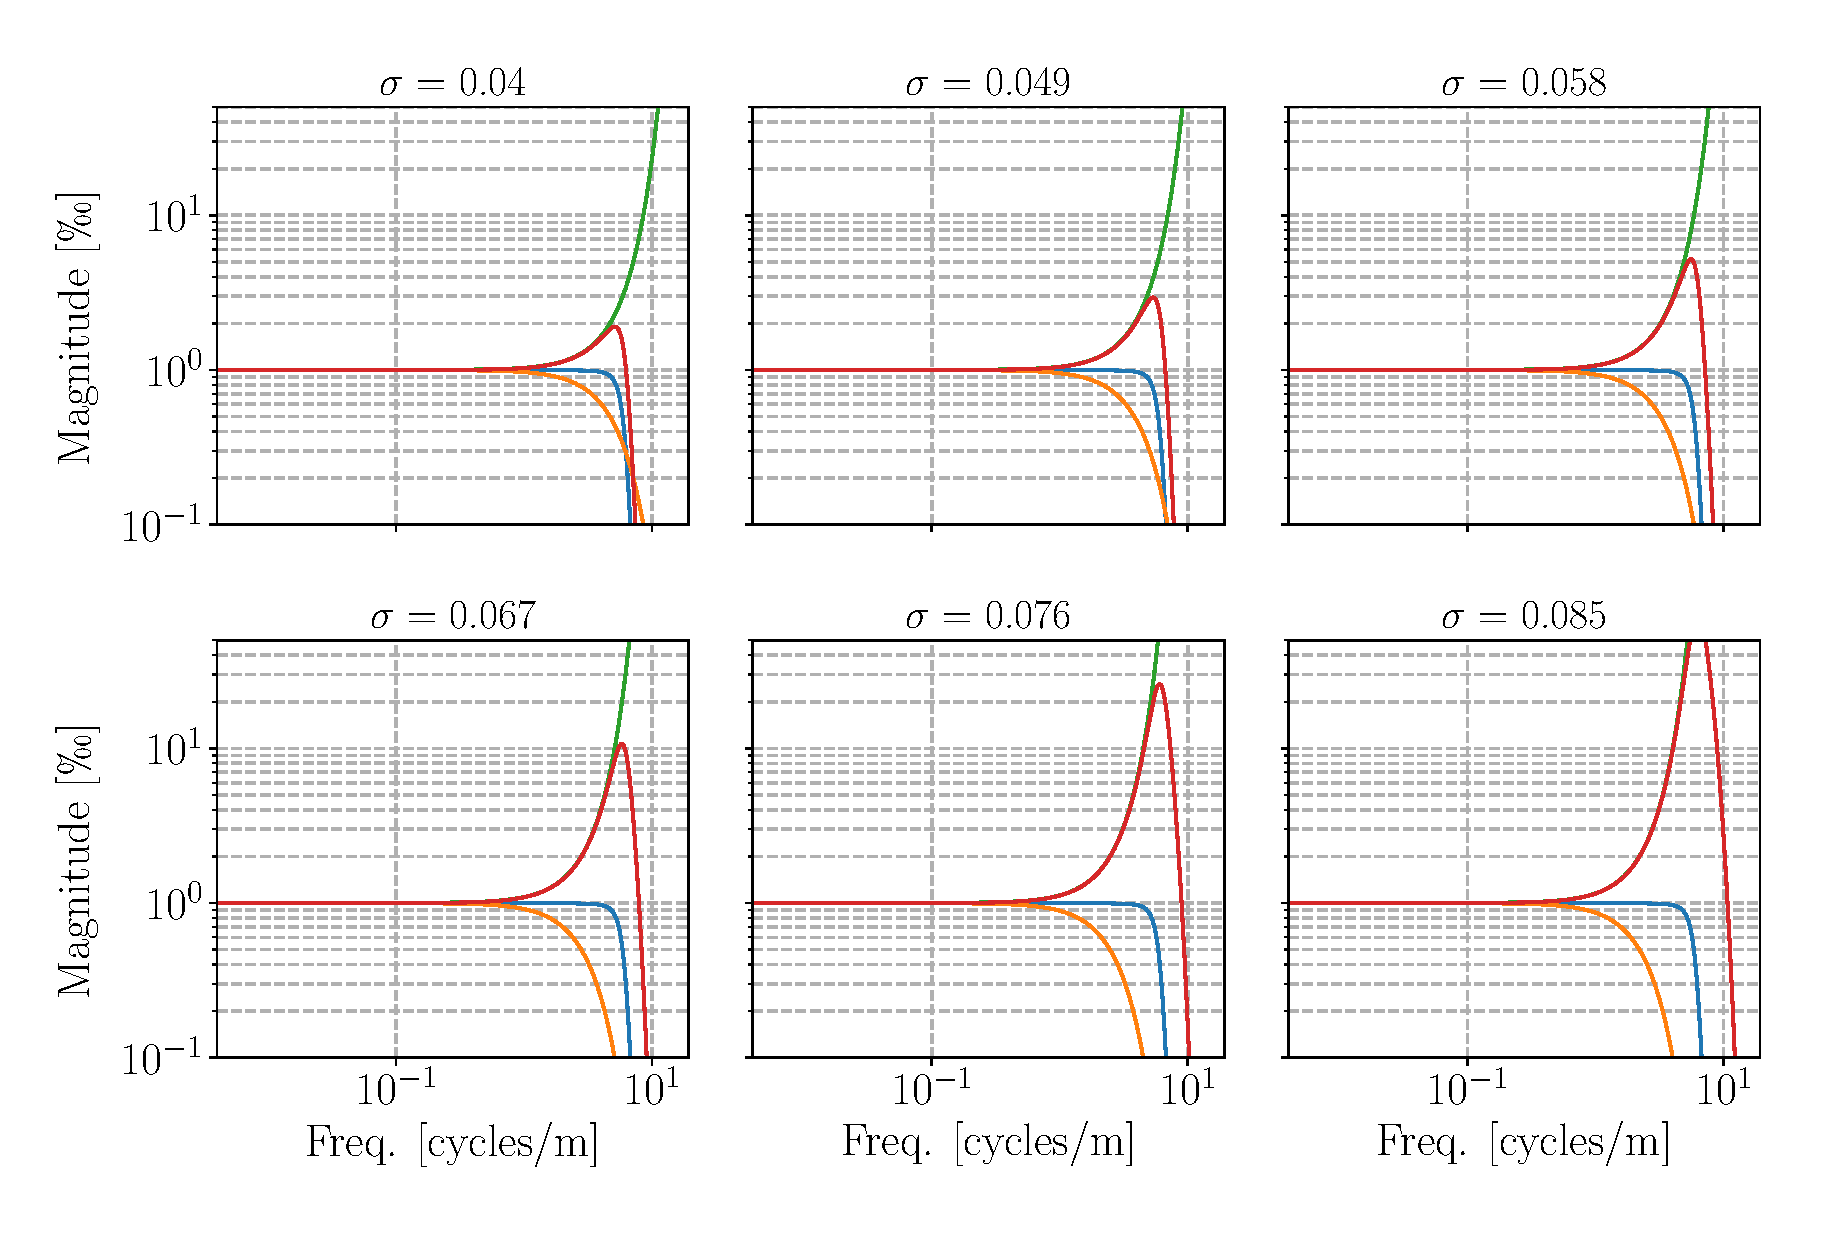
\includegraphics[width=0.9\linewidth]{SiteA_Filters.eps}
	\caption[Filters v. diffusion lengths, Site A]{Frequency filters: The optimal filter found from the PSD (blue), the transfer function (orange), the inverse of the transfer function (green) and the combined signal restoration filter (red).}
	\label{fig:SiteA_Filters}
\end{figure}
}

\frame{
	\frametitle{Deconvolution}
	
\begin{figure}
	\centering
	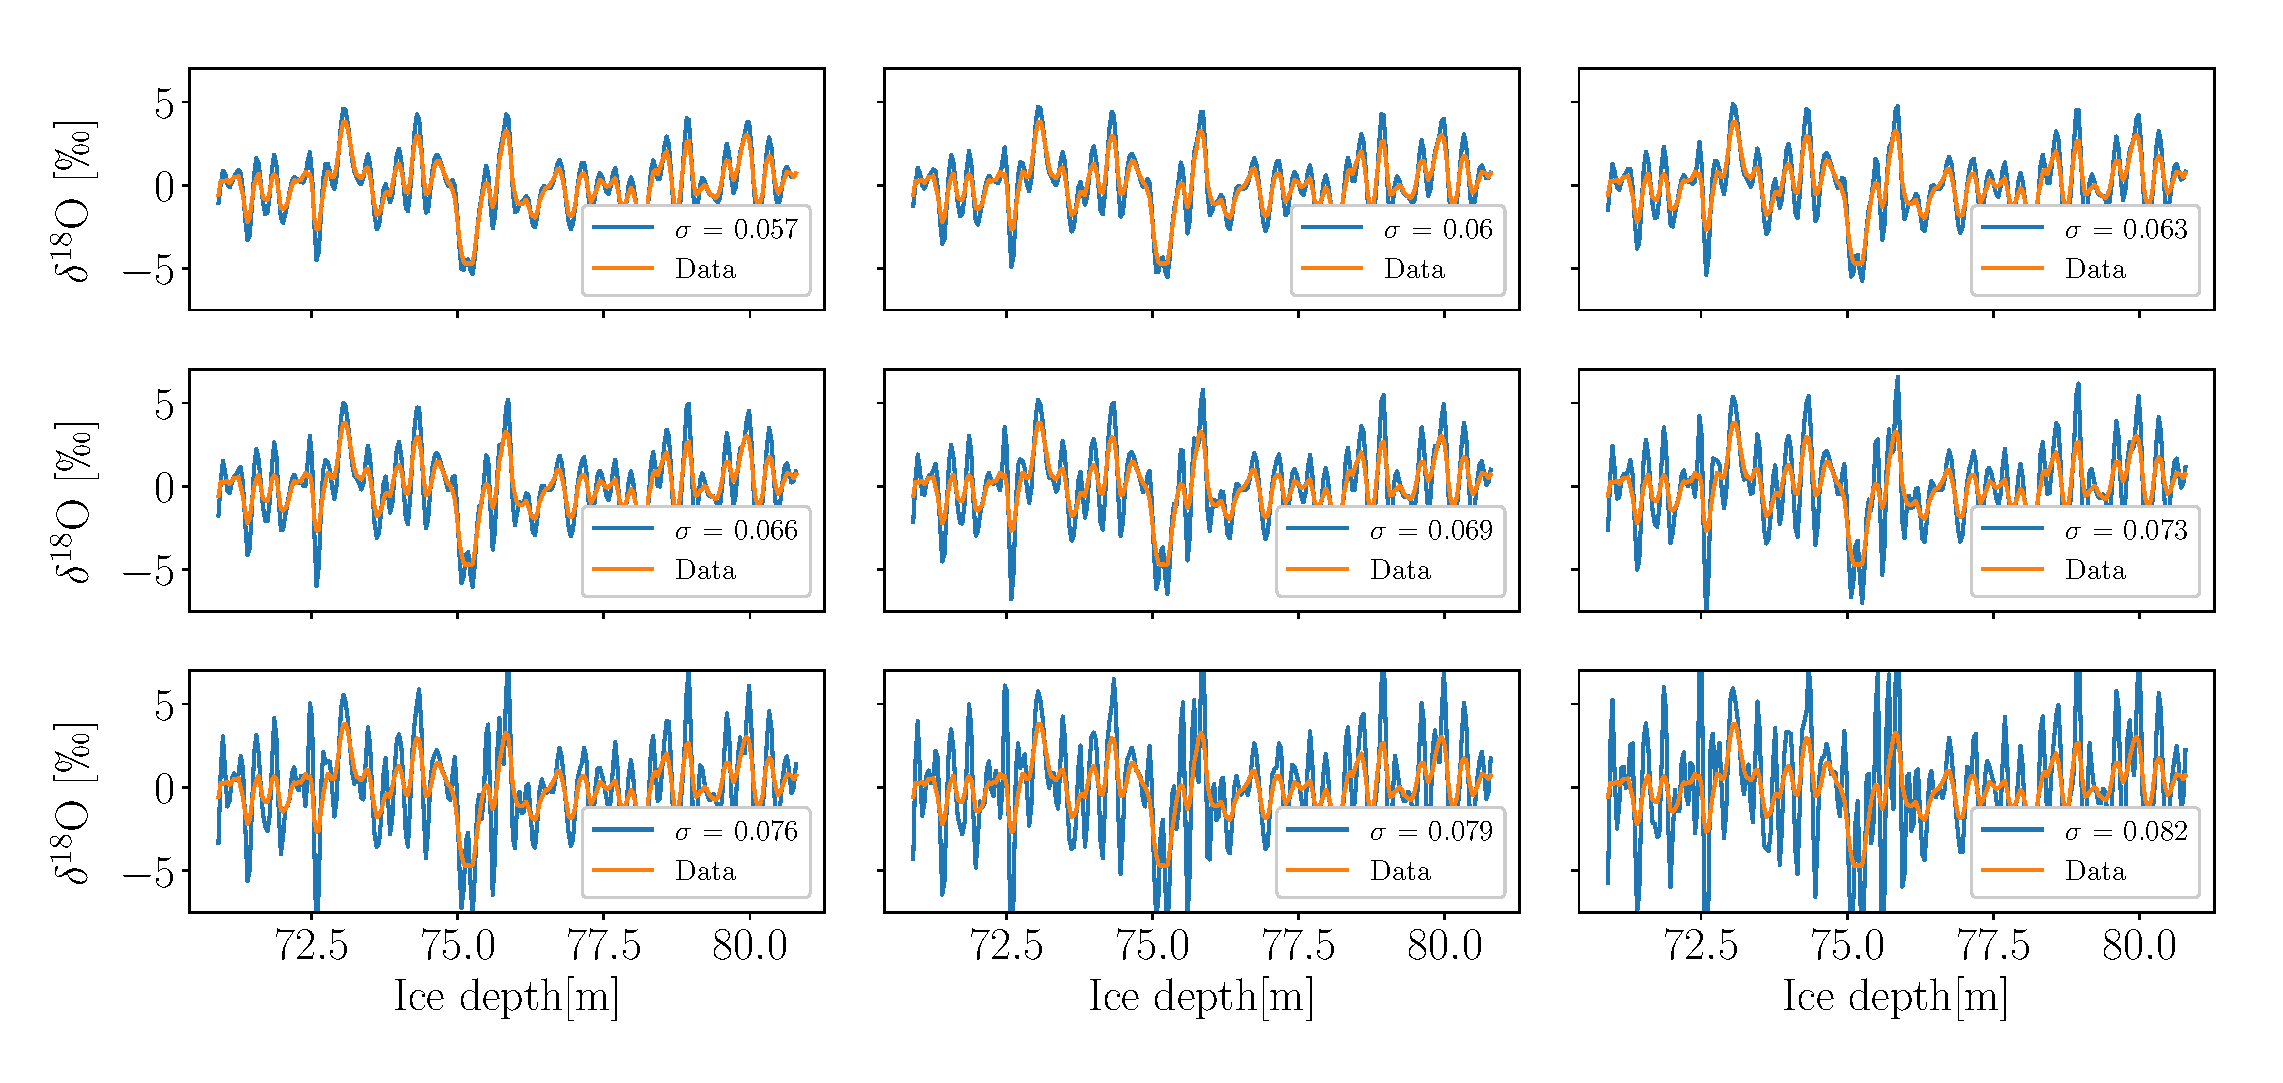
\includegraphics[width=\textwidth]{SiteA_Decons.eps}
	\caption[Restored signals v. diffusion lengths, Site A]{The estimated restored signal (blue) given diffusion length. Plotted along with original measured data (orange).}
	\label{fig:SiteA_Decons}
\end{figure}
}

\frame{
	\frametitle{Enhanced Signal, Minimized Noise}
	
\begin{figure}
	\centering
	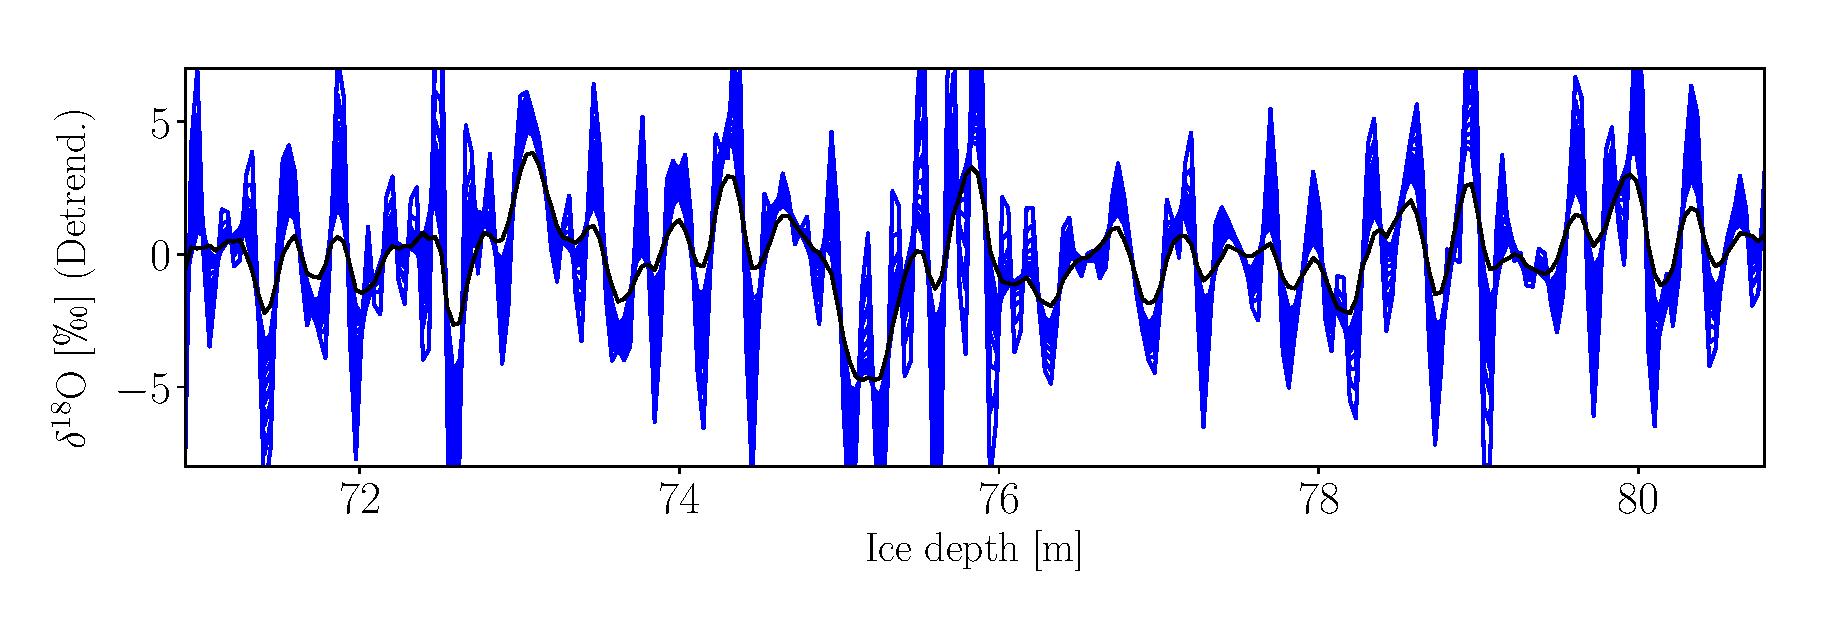
\includegraphics[width=\textwidth]{SiteA_DeconComboAll.eps}
	\caption[Combined restored data, Site A.]{The original data plotted along with each estimate of the restored data with diffusion lengths ranging from 0.057 to 0.085.}
	\label{fig:SiteA_DeconComboFull}
\end{figure}
}

\frame{
	\frametitle{Enhanced Signal, Minimized Noise}
	
	\begin{figure}
		\centering
		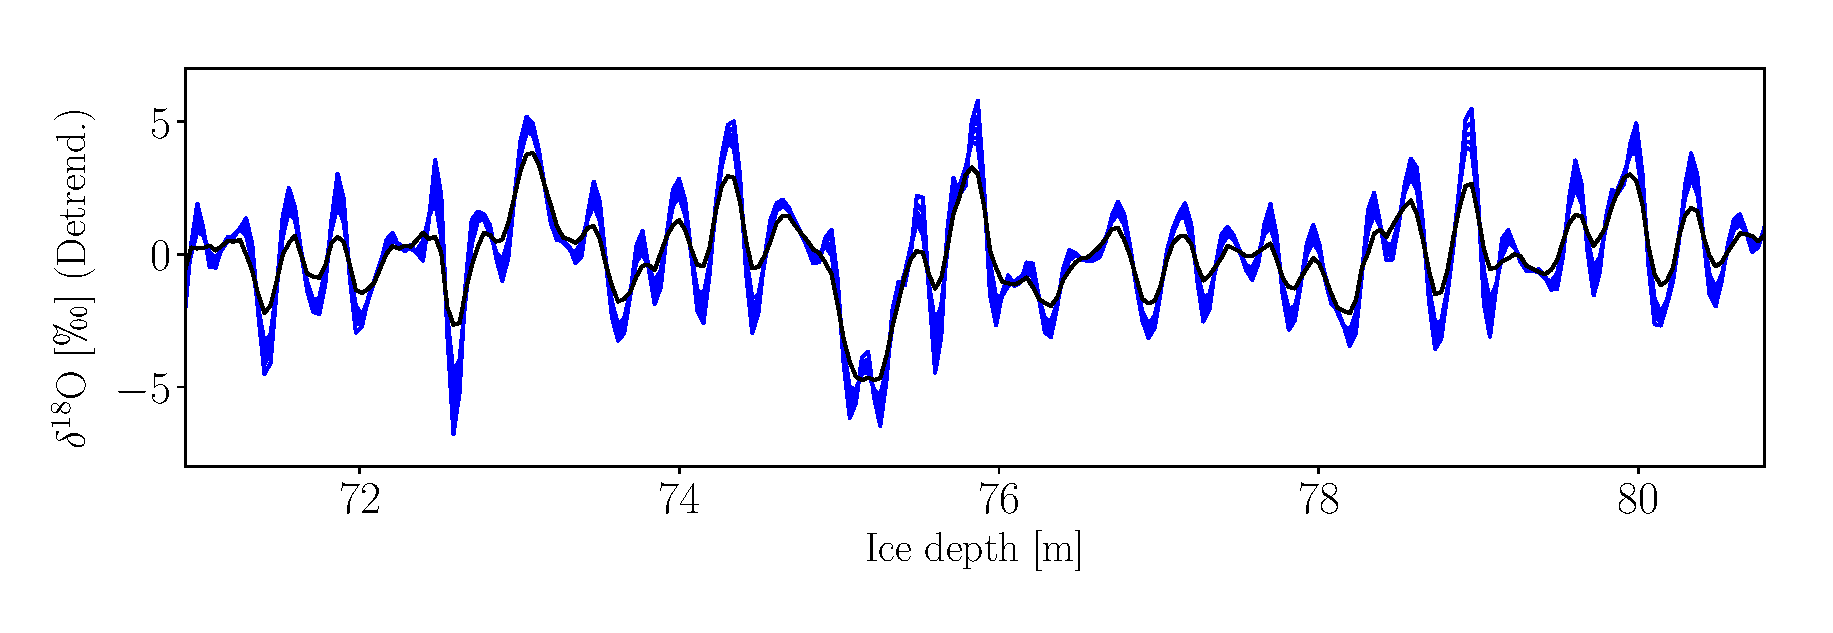
\includegraphics[width=\textwidth]{SiteA_DeconComboFilt.eps}
		\caption[Combined restored data, Site A.]{The original data plotted along with each estimate of the restored data with diffusion length $\sigma^2 < 0.07$.}
		\label{fig:SiteA_DeconComboFilt}
	\end{figure}
}


%\subsection{Measuring Methods}
%
%\frame{
%	\frametitle{Measuring Isotopes}
%	
%}

%\frame{
%	\frametitle{ECM and DEP}
%	
%}









%\subsection{Ice Cores Examined}

%\frame{
%	\frametitle{B-cores (AWI)}
%	
%}

%\frame{
%	\frametitle{Alphabet Cores}
%	
%}

%\frame{
%	\frametitle{Crête, Milcent}
%	
%}









\section{And now?}

\subsection{Detrend and Standardize}

\frame{
	\frametitle{Estimating Cycle Length - ACF}
	\begin{equation}
		R_k = \frac{1}{(n-k)\sigma^2}\sum_{i=1}^{n-k}(x_i - \mu)(x_{i+k} - \mu)
	\end{equation}
	\footnotesize{The estimated cycle length, $l$, will be the first $k$ such that $R_{k-1} > R_{k-2}$ and $R_k < R(k-1)$}
	\begin{figure}
		\centering
		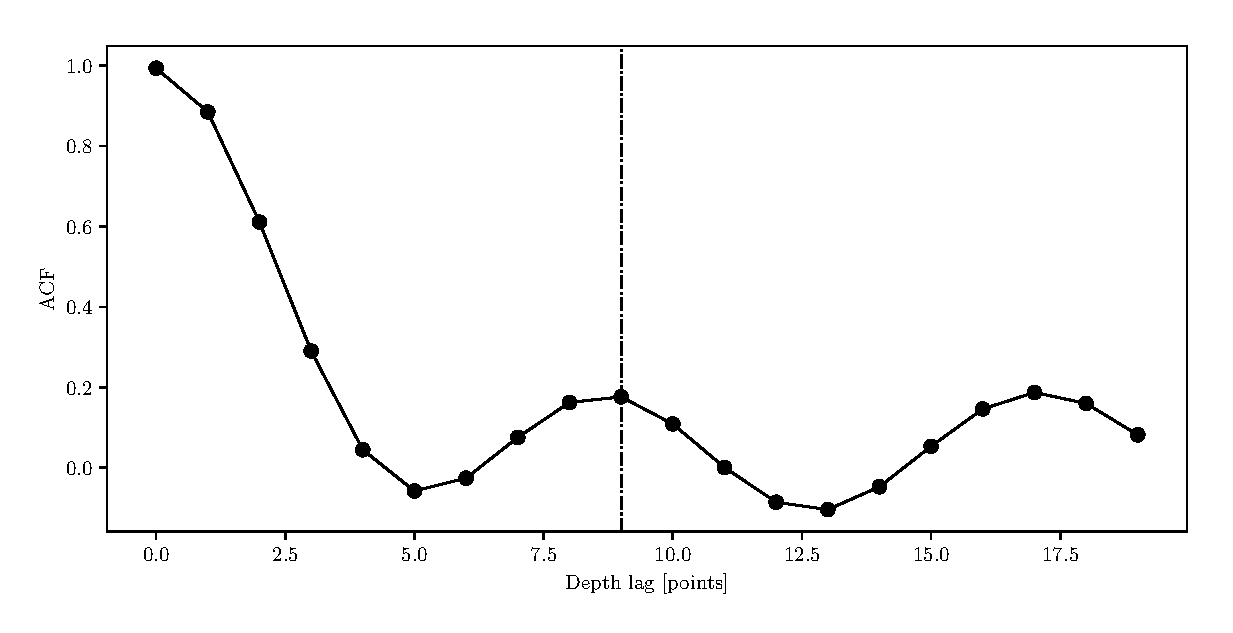
\includegraphics[width=0.7\textwidth]{figACF.eps}
		\caption{Autocorrelation as a function of (pointwise-) depth lag.}
		\label{fig:ACF}
	\end{figure}
	
}

\frame{
	\frametitle{Estimating Cycle Length - Adjustment}
	\only<1>{
	\begin{figure}
		\centering
		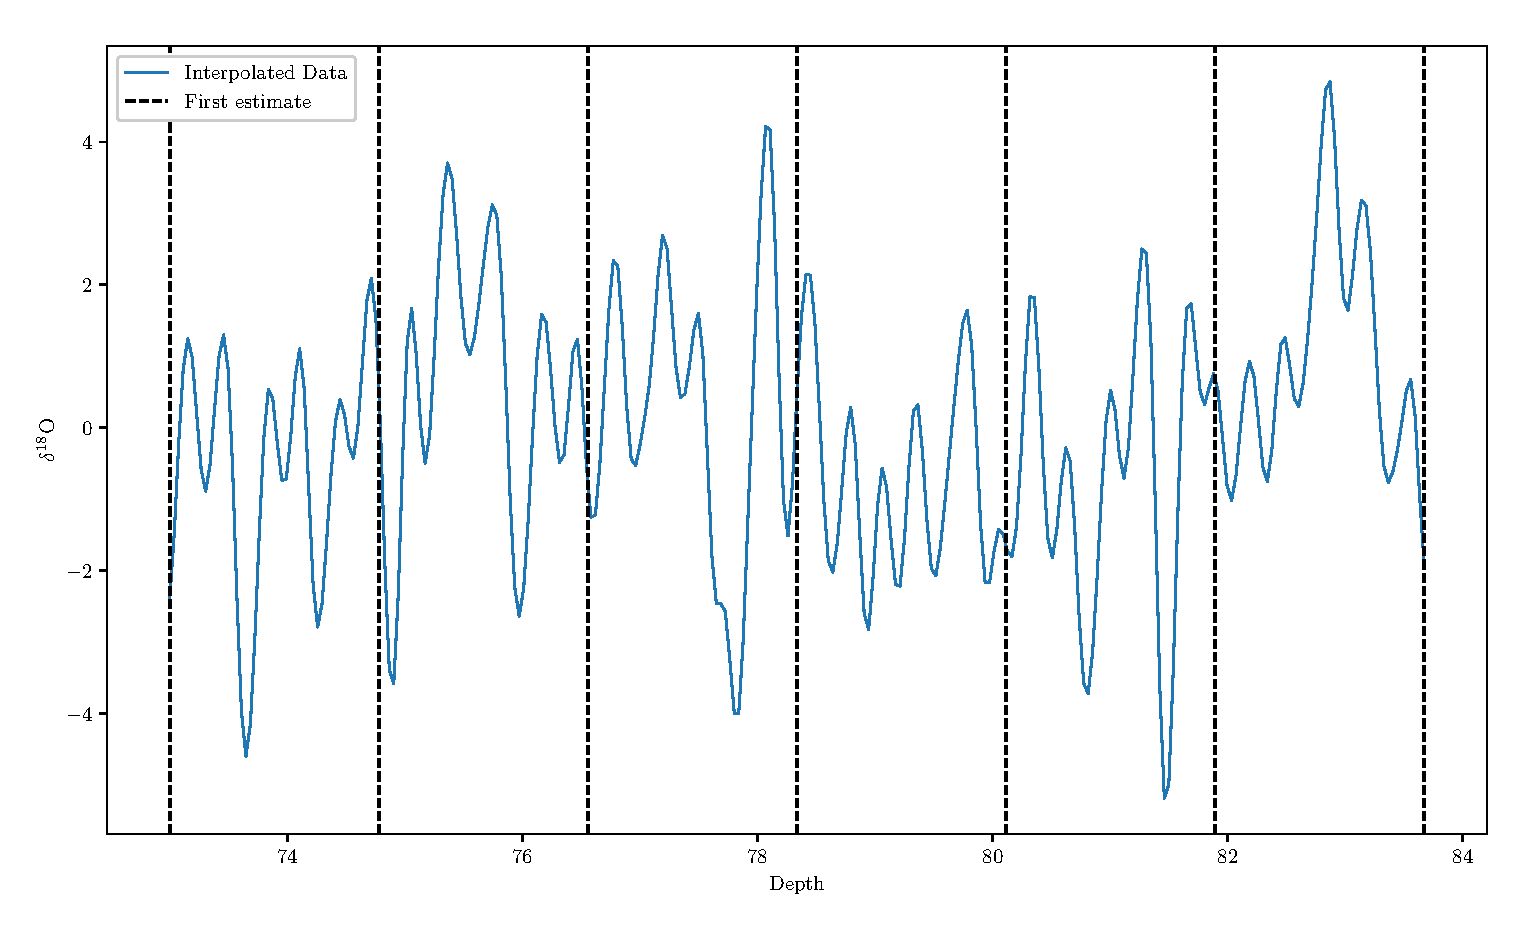
\includegraphics[width=\textwidth]{figCycleEst.eps}
		\caption{First estimate of sections.}
		\label{fig:CycleEst}
	\end{figure}}
	\only<2>{
	\begin{figure}
			\centering
			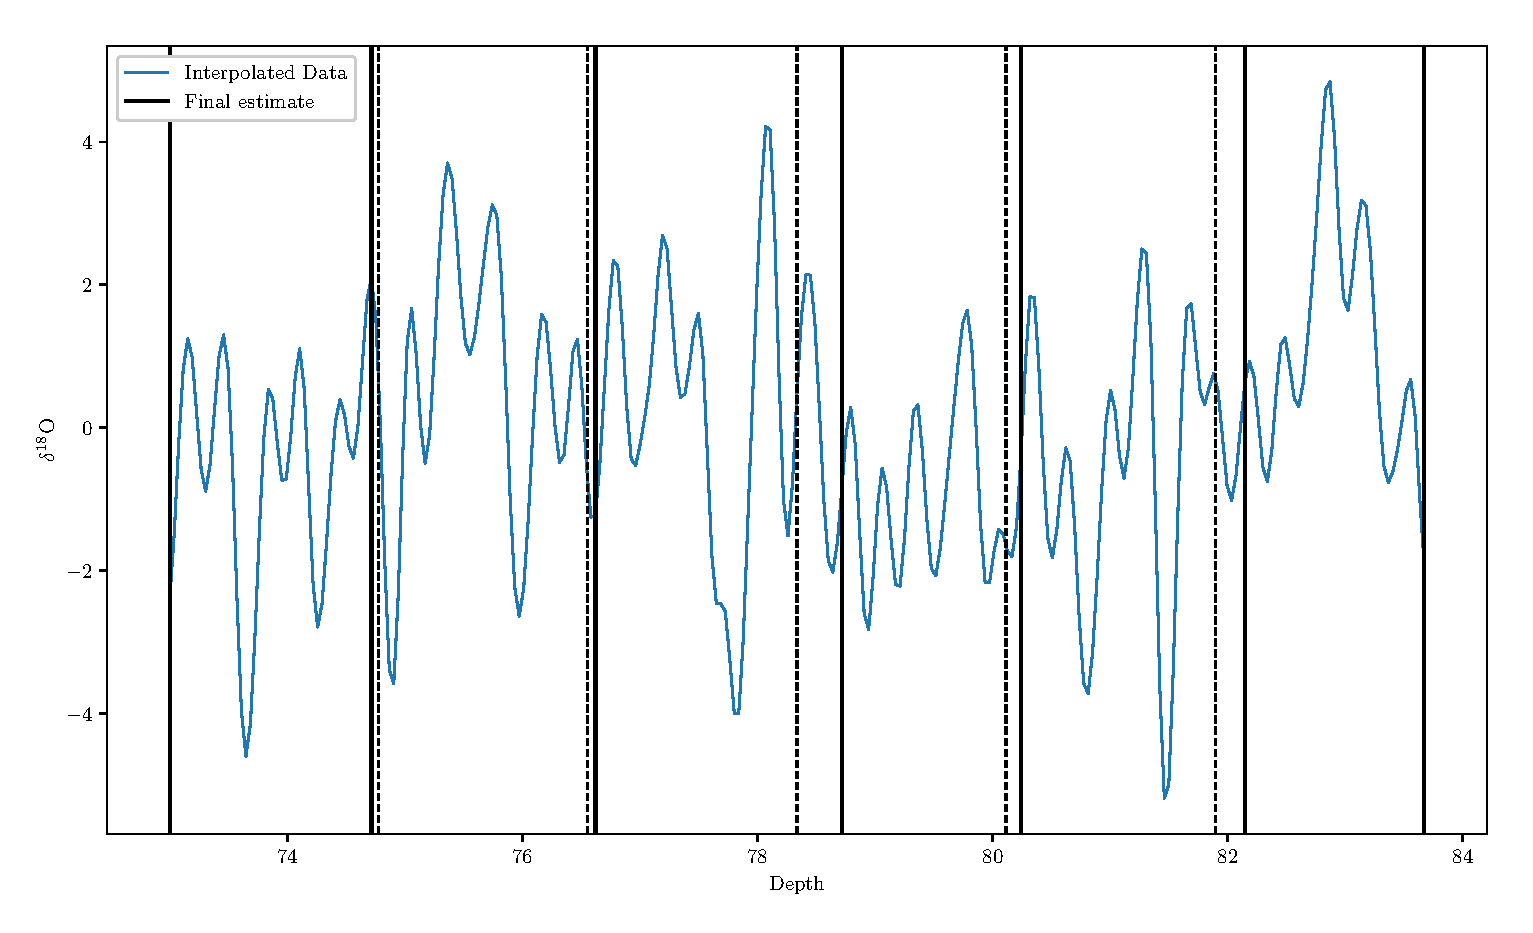
\includegraphics[width=\textwidth]{figCycleEstFin.eps}
			\caption{Final estimate of sections.}
			\label{fig:CycleEstFin}
	\end{figure}}
	
}
\frame{
	\frametitle{Detrending with Moving Average}
	Moving average:
	\begin{equation}
		\mu_i = \sum_{j=i-l_i/2}^{i+l_i/2}\frac{x_i}{l_i + 1}
	\end{equation}
	Moving standard deviation
	\begin{equation}
		\sigma_i^2 = \sum_{j=i-l_i/2}^{i+l_i/2} \frac{(x_i - \mu_i)^2}{l_i + 1}
	\end{equation}
	New standardized signal $\bar{s}$:
	\begin{equation}
		s_i = \frac{x_i - \mu_i}{\sqrt{2}\sigma_i}
	\end{equation}
}
\frame{
	\frametitle{Detrending and standardize}
	\begin{figure}
		\centering
		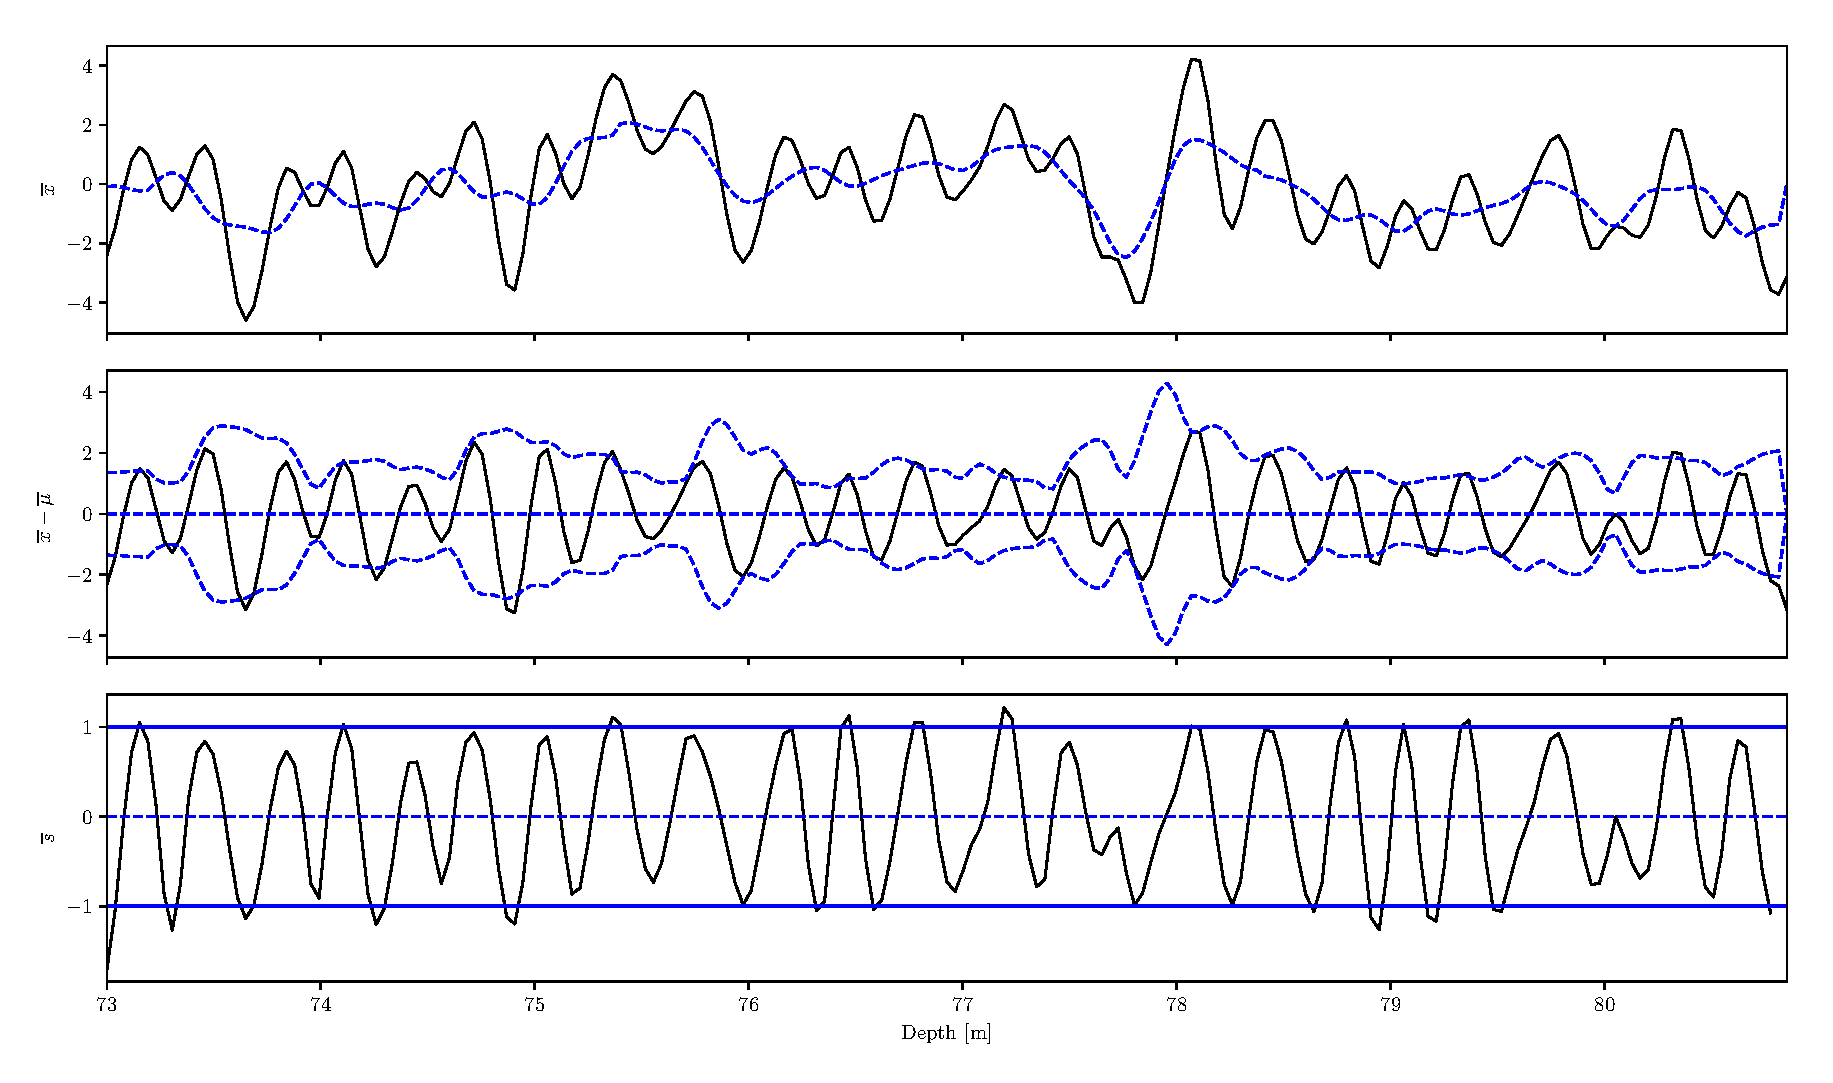
\includegraphics[width=\textwidth]{figStandardized.eps}
		\caption{Standardization through moving average, $\bar{\mu}$, and standard deviation, $\bar{\sigma}^2$}
		\label{fig:Standardized}
	\end{figure}
}






\subsection{Layer Counting Algorithm}

\frame{
	\frametitle{Peak Detection by Pattern Recognition}
	\begin{itemize}
		\item Prior information: Typical annual cycle (noisy sine)
		\item Convolutional Neural Networks 
		\item Kalman Filtering, MCMC or something else entirely
	\end{itemize}
	
}

\frame{
	\frametitle{Layer Counting Algorithm}
	\onslide<1->{Prior to estimation:
	\begin{itemize}
		\item Diffusion and densification models
		\item Noisy sine signal
	\end{itemize}}
	\onslide<2->{Outcome:
	\begin{itemize}
		\item Peak counting
		\item Dating by years
		\item Layer thickness approximation
	\end{itemize}}
}



\section{Outlook}

\subsection{Layer Counting Algorithm, Cont.}


\frame{
	\frametitle{Layer Counting Algorithm}
	\begin{itemize}
		\item In Different Cores, Same (Known) Age
		\item Down entire (Dated) Core
		\item Combination
	\end{itemize}

}


\frame{
	\frametitle{Thank you!}
	\LARGE \textbf{Any questions?}
}


%\appendix
%\begingroup
%\begin{frame}[allowframebreaks]
%\frametitle{References}
%\begin{multicols}{2}
%	
%	\begin{thebibliography}{9}	
%	\end{thebibliography}
%\end{multicols}
%\end{frame}
%\endgroup
%    \begin{itemize}[<+->]
%        \item Something
%        \item Something more
%        \item Something third
%    \end{itemize}
%    \begin{block}{Definition}
%        \only<1>{Travel time is the time required by the particle to move from one point to another point.}
%        \only<2>{Residence time is the time required for the particle to get out of the system.}
%        \only<3>{Biology is the study of living things.}
%    \end{block} 



\end{document}


